\documentclass[../distribution_theory_notes.tex]{subfiles}
\begin{document}
\section{Aula 02 - 19 de Agosto, 2024}
\subsection{Motivações}
\begin{itemize}
	\item Espaços de Fréchet;
	\item Seminormas.
\end{itemize}
\subsection{Espaços de Fréchet}
Podemos dizer que a Teoria das Distribuições é uma parte da análise funcional que se desenvolve separadamente dos espaços de Banach ou de Hilbert, tendo em vista que ela examina espaços duais de certos espaços vetoriais de funções, as chamadas funções ``testes'', cuja maneira natural de convergência é uma que não pode ser descrita por uma norma, mas que, felizmente, ainda é compatível com a estrutura linear dos mesmos, que nos leva ao conceito dos Espaços Vetoriais Topológicos. 

Mesmo não sendo normados, eles possuem algumas propriedades análogas às do espaço normado que são úteis para a obtenção das propriedades que desejamos, tais como: 
\begin{itemize}
  \item[i)] Metrizabilidade: permite o estudo por meio de limites de sequências;
  \item[ii)] Convexidade Local: as bolas, tanto abertas quanto fechadas, são convexas;
  \item[iii)] Possui SFV equilibrado: a origem possui um SFV ``invariante por rotação escalar'' e simétrico com relação à origem; e 
  \item[iv)] Completeza: o que faz deles espaços de Baire, ou seja, isenta a análise da consideração de ``conjuntos insignificantes''. 
\end{itemize}
A classe de TVS que cumpre todos os requisitos acima listados e não necessariamente normado é chamada de \textbf{Espaços de Fréchet}; trataremos deles na aula de hoje.

\begin{theorem*}
  Em um TVS \((E, \tau )\), toda vizinhança U da origem contém uma vizinhança equilibrada da origem.
\end{theorem*}
\begin{proof*}
  Com efeito, como \(M(0, 0)=0 \cdot 0 = 0\in U\), segue da continuidade da multiplicação que existem \(\delta > 0\) e \(V\in \tau \), com \(0\in V\) tais que \(B_{\mathbb{C}}(0; \delta )\times V\subseteq M^{-1}(0)\), ou seja, 
    \[
      |\lambda |<\delta \;\&\; x\in V \Rightarrow \lambda \cdot x\in U.
    \]
    Daí, segue que 
      \[
        B\coloneqq \bigcup_{|\lambda |<\delta }^{}\lambda \cdot V=M(B_{\mathbb{C}}(0; \delta ) \times V) \subseteq U
      \]
      e que B é equilibrado, já que, se \(|\alpha |\leq 1,\; |\alpha \lambda |\leq |\lambda |<\delta \) , então \((\alpha \lambda )V\) está contido em B, isto é, 
        \[
          |\alpha |\leq 1 \Rightarrow \alpha B \subseteq B.
        \] 
 \begin{figure}[H]
 \begin{center}
 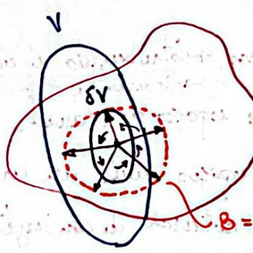
\includegraphics[height=0.5\textheight, width=0.5\textwidth, keepaspectratio]{./Images/open_union_2.png}
 \end{center}
 \caption{o conjunto B é a reunião de todas as rotações de \(\delta V\) ao redor da origem, deixando-o ``redondo''.}
 \end{figure} 

  Finalmente, que B é vizinhança da origem segue do fato de que B é a reunião de abertos: 
    \[
      B = \bigcup_{0<|\lambda |<\delta }^{}\lambda V,
    \]
    conforme o segundo item do Lema 1. 
\end{proof*}
\begin{theorem*}
  Toda vizinhança conexa U da origem de um TVS \((E, \tau )\) contém uma vizinhança da origem convexa e equilibrada.
\end{theorem*}
\begin{proof*}
  Com efeito, primeiramente consideremos uma vizinhança equilibrada da origem B contida em U e notemos que, para \(|\lambda |=1\), tem-se \(\lambda B = B.\) Com isso, se 
    \[
      C\coloneqq \bigcap_{|\lambda |=1}^{}\lambda \cdot U,
    \]
    então, como intersecção de convexos, C é convexo e 
      \[
        B = \lambda B\subseteq \lambda U,\quad \forall |\lambda |=1,
      \] 
      donde segue que B está contido em C, mostrando que o interior de C é não vazio; desta forma, pondo \(V\coloneqq \mathrm{int}(C)\), afirmamos que este é o conjunto do teorema. 

      De fato, V é vizinhança da origem, pois 
        \[
          0\in B\subseteq \mathrm{int}(C)=V;
        \]
        além disso, V é convexo, pois o interior de um convexo é um convexo. Por fim, como U é convexo e 0 pertence a ele, para \(0\leq t\leq 1\) e x em U, tem-se que 
          \[
            tx + (1-t)0\in U,
          \]
          isto é, para \(0\leq t\leq 1\), 
            \[
              tU\subseteq U;
            \]
            logo, dado \(|\alpha |\leq 1\), como \(\alpha =|\alpha |e^{i\theta }\), concluímos que 
              \[
                \alpha C = \bigcap_{|\lambda |=1}^{}(e^{i\theta }\lambda )|\alpha |U = \bigcap_{|\alpha |=1}^{}|\alpha | U \subseteq \bigcap_{|\alpha |=1}^{}U = C.
              \]
              Portanto, C é equilibrado, fazendo com que V, como interior de um conjunto equilibrado, também o seja. \qedsymbol

\end{proof*}

  \begin{tcolorbox}[
  skin=enhanced,
  title=Lembrete!,
  after title={\hfill Interior de Convexo},
  fonttitle=\bfseries,
  sharp corners=downhill,
colframe=black,
  colbacktitle=yellow!75!white, 
  colback=yellow!30,
  colbacklower=black,
coltitle=black,
  %drop fuzzy shadow,
  drop large lifted shadow
  ]
  Para D convexo, tem-se 
    \[
      M_t(\mathrm{int}(D))=\mathrm{int}(M_t(D))\;\text{ou}\; \mathrm{int}(tD)=t \mathrm{int}(D)\in \tau_{E},\; t\neq 0.
    \] 
    Assim, 
      \[
        (1-t)D + tD\subseteq D \Rightarrow (1-t)\mathrm{int}(D)+t \mathrm{int}(D) \subseteq (1-t)D + tD \subseteq D,
      \]
      e, sendo o conjunto à esquerda um aberto, segue que ele está contido no interior de D.
  \end{tcolorbox}

\end{document}
